\documentclass[10pt]{article}

%% Various useful packages and commands from different sources

\usepackage[applemac]{inputenc}
\usepackage[english]{babel}
\usepackage[T1]{fontenc}
\usepackage{cite, url,color} % Citation numbers being automatically sorted and properly "compressed/ranged".
%\usepackage{pgfplots}
\usepackage{graphics,amsfonts}
\usepackage[pdftex]{graphicx}
\usepackage[cmex10]{amsmath}
% Also, note that the amsmath package sets \interdisplaylinepenalty to 10000
% thus preventing page breaks from occurring within multiline equations. Use:
 \interdisplaylinepenalty=2500
% after loading amsmath to restore such page breaks as IEEEtran.cls normally does.

% Compact lists
\usepackage{enumitem}
\usepackage{booktabs}
\usepackage{fancyvrb}

\usepackage{listings} % for Matlab code
\definecolor{commenti}{rgb}{0.13,0.55,0.13}
\definecolor{stringhe}{rgb}{0.63,0.125,0.94}
\lstloadlanguages{Matlab}
\lstset{% general command to set parameter(s)
framexleftmargin=0mm,
frame=single,
keywordstyle = \color{blue},% blue keywords
identifierstyle =, % nothing happens
commentstyle = \color{commenti}, % comments
stringstyle = \ttfamily \color{stringhe}, % typewriter type for strings
showstringspaces = false, % no special string spaces
emph = {for, if, then, else, end},
emphstyle = \color{blue},
firstnumber = 1,
numbers =right, %  show number_line
numberstyle = \tiny, % style of number_line
stepnumber = 5, % one number_line after stepnumber
numbersep = 5pt,
language = {Matlab},
extendedchars = true,
breaklines = true,
breakautoindent = true,
breakindent = 30pt,
basicstyle=\footnotesize\ttfamily
}

\usepackage{array}
% http://www.ctan.org/tex-archive/macros/latex/required/tools/
\usepackage{mdwmath}
\usepackage{mdwtab}
%mdwtab.sty	-- A complete ground-up rewrite of LaTeX's `tabular' and  `array' environments.  Has lots of advantages over
%		   the standard version, and over the version in `array.sty'.
% *** SUBFIGURE PACKAGES ***
\usepackage[tight,footnotesize]{subfigure}
\usepackage[top=2.2cm, bottom=2.2cm, right=1.7cm,left=1.7cm]{geometry}
\usepackage{indentfirst}


\setlength\parindent{0pt}
\linespread{1}

\usepackage{mathtools}
\DeclarePairedDelimiter{\ceil}{\lceil}{\rceil}
\DeclarePairedDelimiter{\floor}{\lfloor}{\rfloor}
\DeclareMathOperator*{\argmax}{arg\,max}
\newcommand{\M} {\mathtt{M}}
\newcommand{\dB} {\mathrm{dB}}

\graphicspath{ {figures/} }

% equations are numbered section by section
\numberwithin{equation}{section}


\begin{document}
\title{Digital Transmission - Homework 2}
\author{Andrea Dittadi, Davide Magrin, Michele Polese}

\maketitle

\section*{Problem 1}

\subsection*{Choice of $N_h$}

In order to determine a suitable length $N_h$ of the impulse response, we consider the noise that we would introduce by performing the truncation of the power delay profile (that corresponds to a truncation of the random impulse response). The given discrete power delay profile of the channel is a sampled version of
$$ \M(\tau) = \frac{1}{\bar{\tau}_{rms}} e^{-\tau / \bar{\tau}_{rms}} $$
that is
$$ \M(iT_C) = \frac{1}{\bar{\tau}_{rms}} e^{-iT_C / \bar{\tau}_{rms}} $$
with $i$ non-negative integer and $T_C = 1$. This quantity must be then normalized in such a way that
$$\sum_{i=0}^{\infty} \M(iT_C) = 1 - C^2 $$
where $C = \sqrt{K / (K+1)}$ is the deterministic component of the first ray (for $i=0$) and $K$ is the Rice factor. Note that we are considering an infinite number of rays, but as a matter of fact MATLAB approximates as zero all values $\M(iT_C)$ for $i > 894$, therefore we stop the summation to 894 (actually 899, LOL).

Knowing that the true impulse response of the channel has random properties described by the power delay profile $\M(iT_C)$ and by the quantity $C$, then we define the quality of the approximation due to truncation as
$$ \Lambda_t(N_h) = \frac{E[||\mathbf{h}||^2]}{E[||\mathbf{\Delta h}||^2]} = \frac{C^2 + \sum_{i=0}^{\infty} \M(iT_C)}{\sum_{i=N_h}^{\infty} \M(iT_C)} $$
where $\mathbf{h}$ is the vector of the impulse response $[h_0(nT_C),~h_1(nT_C),\ldots]$ and therefore
$$ E[||\mathbf{h}||^2] = E[\sum_{i=0}^{\infty} |h_i(nT_C)|^2] = C^2 + \sum_{i=0}^{\infty} \M(iT_C). $$
The noise in the system is
$$ \Lambda = \frac{\M_x E[||\mathbf{h}||^2]}{4 \sigma_w^2} = \frac{\M_x (C^2 + \sum_{i=0}^{\infty} \M(iT_C))}{4 \sigma_w^2} $$
where $\M_x$ is the statistical power of the input signal. Finally, we define the normalized ratio
$$ \Lambda_n (N_h) = \frac{\Lambda_t}{\Lambda} = \frac{4 \sigma_w^2}{\M_x \sum_{i=N_h}^{\infty} \M(iT_C)} $$
to compare the noise of the system with the noise we are introducing by truncating $\M(iT_C)$ to $N_h$ samples.

Looking at the plot of $\Lambda_n (N_h)_{\dB}$ against $N_h$ in Fig.~\ref{fig:p01_lambda_n}, we can maintain that $N_h = 3$ is a good choice, since we have $\Lambda_n(2) \approx 2~\dB$ and $\Lambda_n(3) \approx 5.6~\dB$.

\begin{figure}[ht]
	\centering
	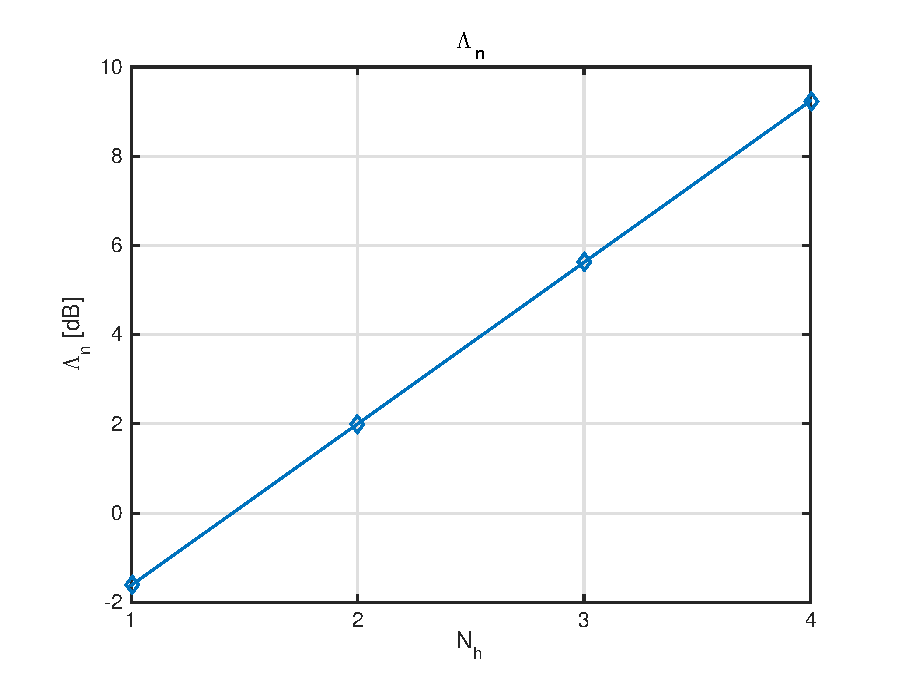
\includegraphics[width=0.52\textwidth]{p01_lambda_n}
	\caption{Plot of $\Lambda_n (N_h)$ in dB for the choice of $N_h$.}
    \label{fig:p01_lambda_n}
\end{figure}

\begin{thebibliography}{10}

\bibitem{bc}
Benvenuto, Cherubini, Algorithms for Communications Systems and their Applications, Wiley, 2004


\end{thebibliography}

\end{document}